\chapter{DISCUSSION}
\label{ch:discussion}

\section{Volume Registration}

The fetal scans were manually segmented, the masks used in the segmentation were created to be uniform across the whole sequence. The intention behind this process is to remove all voxel values not associated with the organ of interest. However, fetal motion is highly variable. It is possible for a subject to rotate in any direction. The subject may drastically change position in the middle of the scan, possibly several times. The manually created masks were developed using a software tool which allows 3D image masks to be applied to an entire 4D image sequence. The masks were required to be created to ensure the fetal brain or placenta would be inside the masked area at all times. The masks may cover some area that does not belong to the organ of interest.

This limitation is unique to the fetal images. Existing pre-processing pipelines exist for skull stripping for neonatal and preadolescent images. Development of a similar pipeline for fetal images, while a challenge, would make research surrounding fetal rs-fMRIs more accessible to the medical imaging community.

Alternatively, the field of computer vision offers some SOMETHING.

\textbf{Registration fixes positional effects of motion, not spin history or susceptibility effects}
Subject motion during rs-MRI scans affects both the recorded position and orientation of the subject as well as the established magnetic spin gradients within the skull. The DAG-based technique can correct the positional effects of motion, but it cannot correct the effects of the motion that disrupt the magnetic spin gradients. Methods for prospectively estimating subject motion exist and can be used to change slice positions in each volume during acquisition. Retrospective techniques to correct for this effect will require shot-to-shot modeling of macroscopic $B_0$ fields and are beyond the scope of the present research.

\section{Characterizing Motion}

The models used to characterize motion were able to identify the differences between general patient age group based on the metrics used to measure motion in the original sequences.

Additional analyses could be performed to further evaluate the computer detectable differences in patient groups. The models presented in the previous chapter were generated each using a single metric type. Each metric only measures one property of the image volumes. It is possible that combinations of metrics measuring different properties could be used to better separate patient groups. For example, the combination of the FD values which measure the positional changes due to motion and the DVARS values which measure overall signal changes could be combined to comprehensively categorize subjects based on the effects of motion, BOLD signal change, and background noise.



\section{Relation to Existing Work}

\subsection{MRI Simulations} 

The idea of simulated MRIs originated in the 1980s. Bobman et al. suggested a process of MR image synthesis, then demonstrated its validity by creating synthetic spin-echo brain MRIs and comparing the simulated images to clinical images \cite{Bobman1985}. Since then, a number of MRI simulation softwares have been developed. Herein, we discuss two of these tools and compare them to our simulation tool.

The FMRIB group developed a simulation tool called \href{https://fsl.fmrib.ox.ac.uk/fsl/fslwiki/POSSUM}{POSSUM} (Physics-Oriented Simulated Scanner for Understanding MRI) \cite{Drobnjak2006} \cite{Drobnjak2010}. POSSUM offers realistic, physics-based simulation of structural, functional, and diffusion tensor images. It requires a gradient echo pulse sequence and a segmented object with known tissue properties as inputs for the simulation. It allows the user a high degree of control over the physical properties to be simulated. The user has the ability to specify the pulse sequence information, the method for generating brain signal, the addition of motion and noise, and the method for image reconstruction. Both a GUI and a command line interface are available for POSSUM. 

\begin{figure}
\centering
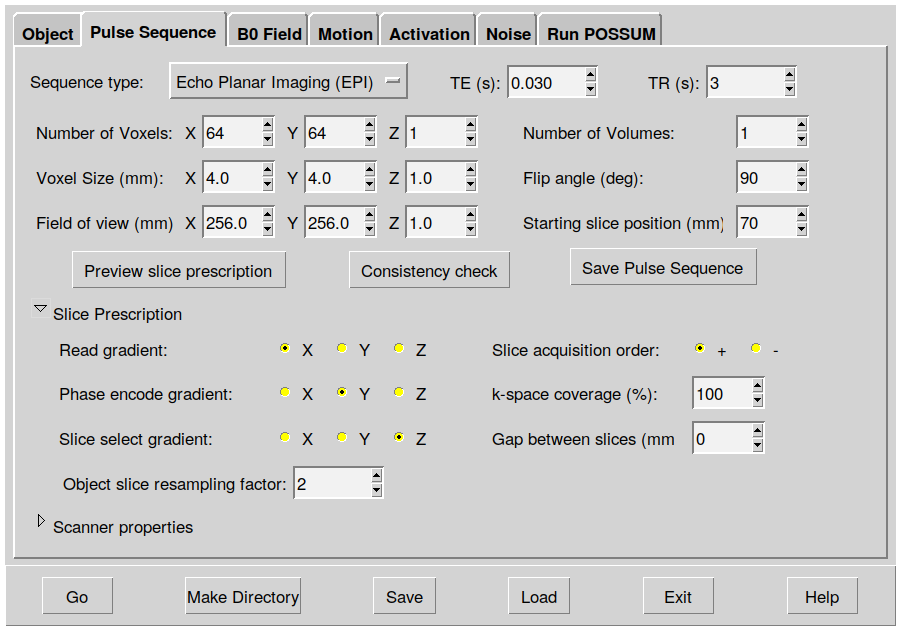
\includegraphics[width=.6\textwidth]{7/possum-gui.png}
\caption{The ``Pulse Sequence'' specifications page in the POSSUM GUI}
\label{fig:possum}
\end{figure}

The biggest drawback to POSSUM is the degree of MR physics knowledge needed to use it effectively. For MR physicists, specifying the details of a pulse sequence may be trivial. For researchers from other fields, customizing pulse sequence parameters, an example of which can be seen in Figure \ref{fig:possum}, can be a challenging task. These customizations may even be unnecessary depending on the goals a researcher hopes to achieve using the simulated data.

If a researcher's goal is to test the impact of a new MRI processing technique on known signals in an image, the BrainWeb MRI simulator might be a better option than POSSUM. BrainWeb was created and is actively developed by the \href{mcgill.ca/bic/}{McConnell Brain Imaging Centre} at McGill University to assist in validation computer-aided MRI analysis tools \cite{kwan1999mri} \cite{collins1998design} \cite{cocosco1997brainweb} \cite{kwan1996extensible}. A set of simulated images have been generated using BrainWeb and are can be found in the BrainWeb Simulated Brain Database (SBD). The SBD contains simulated images for healthy subjects and for subjects who have lesions due to multiple sclerosis.

Custom simulations can be generated on the BrainWeb server by submitting a request via a browser. The simulation request form has three areas which can be customized: the type of brain to simulate, the MR pulse sequence, and the imaging artifacts. The simulation is run on the server and the user is notified via email when the simulated images are ready to download. 

BrainWeb's simulator is slightly more approachable than POSSUM: a limited number of pulse sequence parameters are available to customize and a description is listed next to each parameter in the pulse sequence and imaging artifacts sections. However, the user has slightly less control over the simulated image. The brain models used by BrainWeb are healthy brains or brains with MS lesions. It is not an option for the user to upload an image to use as the structural information in the sequence. For our purposes, the biggest limitation of BrainWeb is that it only simulates structural images. 

Our simulation tool, SPECTr, is one of the few tools which simulates resting-state fMRIs. It offers the opportunity for researchers to explore the effects of their motion correction techniques on BOLD signal, background noise, and patient motion using a lightweight simulation that can be run on a personal computer. It should be noted that SPECTr is not a substitute for the physics-based models in POSSUM and BrainWeb: it is intended to evaluate signal changes in rs-fMRI sequences as a result of post-acquisition image processing.

\subsection{Volume Registration} 

To the best of our knowledge, the only other study that has used a variant of the DAG-based method was performed by Liao et al \cite{Liao2016}. Liao et al’s dataset consisted of 10 fetal rs-fMRIs. In each of these sequences, the fetal brain, fetal liver, and placenta were manually segmented in the first volume of the sequence as well as in five other randomly chosen volumes. These overlap of these manual segmentations before and after registration as measured using the Dice coefficient was used to quantify the amount of motion in each sequence. Even though the Dice coefficients increase more in each sequence after Liao et al.’s registration than after traditional registration, their measure of positional change fails to quantify any changes in position between any other pairs of volumes that do not have manual segmentations. 

\subsection{Age Group Specific Motion}

Satterthwaite et al. note that motion is often correlated with patient age in adolescent populations and specifically designed a study of adolescents ages 8-23 such that patient age and motion were uncorrelated (Satterthwaite 2012a?).